\documentclass{article} 
\usepackage{todonotes}
\usepackage{graphicx}
\usepackage{algorithm}
\usepackage[noend]{algpseudocode}
\usepackage{float}
\usepackage[font=small,labelfont=bf]{caption}
\usepackage[left=0.8in, right=0.8in, top=0.9in, bottom=1in]{geometry}
\usepackage{hyperref} 
%\usepackage{caption}
\graphicspath{ {images/} }


\title{ \textbf {\vspace{0.5cm}\Huge TinyCoin: Simulating mining strategies in a simplified Bitcoin Network\\ \vspace{0.5cm}}
 Final Project for the Peer to Peer course \vspace{1.0cm}\\} 

\date{\vspace{1.7cm}}

\author{ \Large Francesco Balzano \vspace{0.3cm}\\ 
%Matricola 541533 \vspace{0.5cm}\\
\Large Master Degree in Computer Science and Networking \vspace{0.4cm} \\
\Large A.Y. 2016-2017 
}


\begin{document}
  \pagenumbering{gobble}
  \maketitle
  %\newpage
  \noindent\rule{18cm}{0.4pt}
  \tableofcontents
  \newpage
  \pagenumbering{arabic}

\clearpage
\setcounter{page}{2}
  
\section{Overview}  
In this project I have implemented a simplified version of Bitcoin, called TinyCoin, whose specifications are reported in [1]. In brief, TinyCoin distinguishing features are:
\begin{itemize}
\item each user has a single address that records the unspent amount at that node
\item each transaction has a single input, a single output and does not include neither a digital signature nor scripts
\item network nodes may be either normal nodes or miners. In turn, miners may be either honest or fraudolent (\textit{i.e. Selfish Miners}). Each miner has a type that reflects its mining hardware: CPU, GPU, FPGA or ASIC
\item there is a centralized oracle that decides which miner has created a new block of the blockchain at regular intervals of time. The decision is biased by the computational power of the miners. Each block is unique. \\
\end{itemize}
The goal of this project is to evaluate the selfish mining strategy defined in [2] in TinyCoin. This strategy is evaluated by taking into account different metrics and parameters. The results and the discussion of this experiment are reported in the \textit{Results} section.

\section{Design choices}
In the following subsections I explain the design choices that I made. This is a high level description, indeed the classes of the project are described in the \textit{Implementation} section.



\subsection{Network Nodes} Any node in the TinyCoin network is either a (normal) node, or a (honest) miner or a selfish miner. According to the specifications, I have considered a static topology, which is generated at random at the beginning of the simulation.
\begin{itemize}
\item \textbf{node}: makes and receives transactions
\item \textbf{miner}: makes and receives transactions and mines blocks of the blockchain. In particular, as soon as a new block is mined it is immediately advertized to all the nodes in the network.
\item \textbf{selfish miner}: makes and receives transactions and mines blocks of the \textit{private} blockchain. A selfish miner indeed holds both a copy of the public blockchain, which is the ``official'' blockchain, and a copy of the private blockchain, which is the blockchain created and maintained collectively by all the selfish miners. At any time the two blockchains may be equal or may differ for some block. If they differ, it is because the selfish miners have discovered new blocks which have been added to the private blockchain but have not been disclosed to the public. Indeed when a selfish miner mines a new block, it does not naively publish it and add to the public blockchain. Instead, it applies a strategy that allows it and the other selfish miners to get the maximum revenue from their computing power. One of the strategies that they can follow is explained in [2]. In this project, I chosed to implement it. The pseudocode is reported in algorithms \ref{sm_init}, \ref{sm_block} and \ref{sm_others}. \\
\textbf{Initialization} Since we assume that all the nodes are present at the beginning of the simulation, at initialization (algorithm \ref{sm_init}) a selfish miner has both the private and public blockchain empty, and the \textit{privateBranchLength}, which tells how many blocks the two blockchains differ for, is set to zero. \\
\textbf{Selfish Miner found a block} Algorithm \ref{sm_block} describes what happens when one selfish miner creates a new block: the block is added to the private blockchain and the \textit{privateBranchLength} is incremented accordingly. If there was a fork in the public blockchain (line 4), then the selfish miners are in competition with the honest miners to insert their own blocks in the final version of the blockchain. In this case the new block is advertized to all the nodes of the network. In so doing, the selfish miners are quite confident that their two blocks will be included in the blockchain, at the expense of the block mined by the honest miner. Figures \ref{fig:fork}, \ref{fig:fork_2b} and \ref{fig:fork_resolved} illustrate this situation. \\
\textbf{Other miners found a block} Algorithm \ref{sm_others} describes the behaviour of the selfish miner when a (honest) miner creates a new block. If the private blockchain and the public one are equal (line 3), then the selfish miner is fallen behind the other miners and thus accepts the new block and continues mining on top of it. If the selfish miner was one block ahead (line 6), then it advertises to all the nodes its private block, leading to a fork in the blockchain. If the selfish miner was two blocks ahead (line 8), then it publishes both its blocks. This way, it is quite confident that these two blocks will become part of the blockchain, because the branch that it creates is longer than the branch created by the honest miner. If the selfish miner had an advantage of more than 2 blocks (line 11), then it publishes only the first unpublished private block, leading the honest miners to spend clock cycles to mine blocks that at the end won't be part of the final blockchain.
\end{itemize}





\subsection{Blockchain, Blocks and Transactions} 
\begin{itemize}
\item \textbf{transaction}: transactions are generated by nodes. They have an input node, an output node, an amount and a fee. For the sake of simplicity, I have assumed that each node pays the transaction at the moment of creation, and that for each transaction the fee is fixed in percentage.
\item{\textbf{block}}: a block basically contains a list of transactions. For the sake of simplicity, I assumed that the reward for the block creation is immediately given to the miner. If such block is later removed from the blockchain, then also the reward given to the miner is given back. The block creation is arbitrary: it is not required to the miners to solve any Proof Of Work, instead it is the oracle that chooses at random the miner that has to create the new block of the blockchain. 
\item{\textbf{blockchain}}: a blockchain is a list of blocks. It does not include hash pointers, so it is not tamper-free. A block is added to the blockchain if it has been created by a miner and if its parent matches the current last block of the blockchain.
\end{itemize}

\subsection{Forks} 
Forks have a serious impact on the selfish mining strategy. Indeed, selfish miners goal is basically to fork the blockchain, creating a branch that eventually becomes longer than the ``official'' one and thus gets included in the blockchain, to the detriment of the branch created by honest miners. There are two kinds of forks that are supported in this project:
\begin{itemize}
\item \textbf{selfish miner}: it supports forks of arbitrary length, that is the public and the private blockchain may differ for an arbitrary number of blocks from the point of view of the selfish miner. This fact is necessary in order to apply its strategy, as described in algorithms \ref{sm_init}, \ref{sm_block} and \ref{sm_others}.
\item{\textbf{node}}: a normal node only supports a simplified kind of fork, that is one in which there are two branches made of only one block. The next block that is received by the node that extends one of the two branches actually resolves the fork. If at this point another blocks arrives willing to extend the abandoned branch, it will be simply discarded. There are two reasons for this assumption. The first is simplicity: at any time there are no orphan branches in the blockchain, but only a simple fork is admitted. The second is tamper resistance: since the blockchain is not tamper-free, avoiding to leave branches in the blockchain and allowing to fork only the last block of the blockchain means that fraudolent miners cannot mine on top of arbitrary branches instead of the ``official'' one.  
\end{itemize}

\subsection{Network Latencies} 

\begin{algorithm}
\caption{Selfish Miner initialization}\label{sm_init}
\begin{algorithmic}[1]
\State public chain $\gets \emptyset$
\State private chain $\gets \emptyset$
\State privateBranchLength $\gets$ 0
\State Mine at the head of the private chain 
\end{algorithmic}
\end{algorithm}

\begin{algorithm}
\caption{Selfish miners found a block:}\label{sm_block}
\begin{algorithmic}[1]
\State $\Delta\textsubscript{prev}$ $\gets$ length(private chain) - length(public chain)
\State append new block to private chain
\State privateBranchLength $\gets$ privateBranchLength + 1
\If{($\Delta\textsubscript{prev}$ = 0 AND privateBranchLength = 2)}  
\State private chain $\gets$ public chain
\State privateBranchLength $\gets$ 0
\EndIf 
\State Mine at the new head of the private chain 
\end{algorithmic}
\end{algorithm}

\begin{algorithm}
\caption{Honest miners found a block:}\label{sm_others}
\begin{algorithmic}[1]
\State $\Delta\textsubscript{prev}$ $\gets$ length(private chain) - length(public chain)
\State append new block to public chain
\If{($\Delta\textsubscript{prev}$ = 0)}  
\State private chain $\gets$ public chain
\State privateBranchLength $\gets$ 0
\ElsIf{($\Delta\textsubscript{prev}$ = 1)} 
\State{publish last block of the private chain}
\ElsIf{($\Delta\textsubscript{prev}$ = 2)}
\State{publish all of the private chain}
\State{privateBranchLength $\gets$ 0}
\Else 
\State{publish first unpublished block of the private blockchain} 
\EndIf 
\State Mine at the new head of the private chain 
\end{algorithmic}
\end{algorithm}

\begin{figure}
\centerline{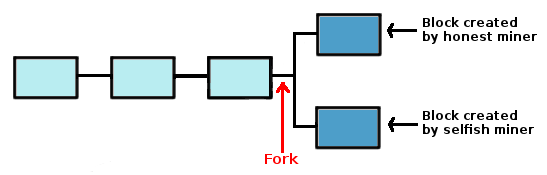
\includegraphics[scale=0.41]{fork}}
\caption{When two different blocks are generated having the same parent (usually these two blocks are generated very close in time), a fork is created in the blockchain.}
\label{fig:fork}
\end{figure}

\begin{figure}
\centerline{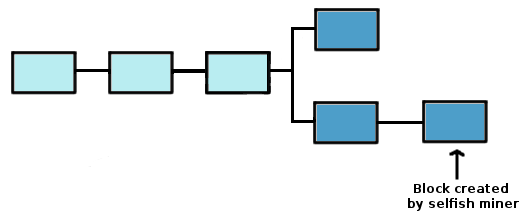
\includegraphics[scale=0.41]{fork_2b}}
\caption{When a selfish miner creates a new block, it adds it immediately to the public blockchain if and only if there is a fork in the blockchain. This way, selfish miners are one block ahead with respect to other miners, and so the probability that their two blocks will be part of the final blockchain increases.}
\label{fig:fork_2b}
\end{figure}

\begin{figure}
\centerline{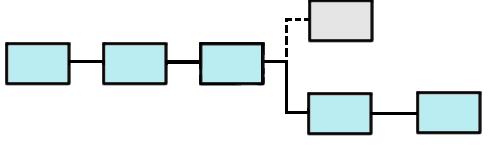
\includegraphics[scale=0.41]{fork_resolved}}
\caption{Selfish miners have reached their goal: their branch is the longest, and so all the miners that were mining on the shorter branch abandon it and start mining on the other, longer branch.}
\label{fig:fork_resolved}
\end{figure}


\section{Implementation}  
I set up the simulation using the event driven version of the Peersim simulator. The classes of this project are in some way dictated by the framework itself. For instance, I wished to have three different classes Node, Miner and SelfishMiner that extended the base class NetworkNode. Each network node would have been one among Node, Miner and SelfishMiner, so that it was immediately clear which was its role in the network. Anyway this was not possible because I had to follow the structure of classes defined by the framework. In this section, I describe the classes that I developed with reference to their role in the framework.
\subsection{Protocols}
Every node in the network is a TinyCoinNode. If the node is a normal node, only the NodeProtocol is enabled; if it is a miner, both the NodeProtocol and the MinerProtocol are enabled; if it is a SelfishMiner, both the SelfishMinerProtocol and the NodeProtocol are enabled (figure \ref{fig:protocols}).
\begin{figure}
\centerline{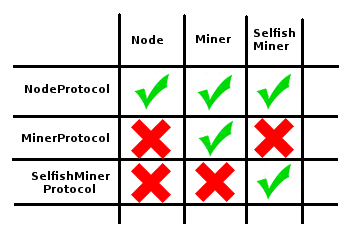
\includegraphics[scale=0.50]{protocols}}
\caption{Relationships between node types and node protocols.}
\label{fig:protocols}
\end{figure}
\begin{itemize}
\item \textbf{NodeProtocol} The NodeProtocol is responsible for creating and advertising transactions and for publishing blocks of the public blockchain. The method \textit{nextCycle()}, called at every cycle, creates a transaction with a fixed probability defined in the configuration file. Both the amount and the recipient of the transaction are random. Then it is published on the network. The method \textit{processEvent()} is invoked every time the NodeProtocol receives a message. A message may be either a transaction or a block. In the former case, if the node hasn't already seen it, it adds the transaction to its transaction pool and floods it to its neighbors. In the latter case the behaviour is different based on the type of node. If the node is a normal node or a honest miner, it checks whether the received block has to be added to the blockchain, checks the eventual presence of forks, makes some other operations and finally floods the block to all its neighbors. Else, if the node is a selfish miner it implements the algorithm \ref{sm_others}. The fact that also the selfish miners run the NodeProtocol could seem weird, but actually there are two reasons for this choice. First: a selfish miner is also a node, able to make and receive transactions. Second: I use the NodeProtocol as a ``public layer'' to exchange public information among the nodes of the network, namely transactions and blocks of the public chain. Instead, I use the SelfishMinerProtocol as a ``private layer'' to exchange private information inside the selfish miners pool, namely the blocks of the private blockchain not disclosed to public yet. 
\item \textbf{MinerProtocol} The MinerProtocol is run by the miners. At each cycle it is invoked the method \textit{nextCycle()}, which is actually executed only if the oracle selected this miner for the current cycle. If this is the case, the miner picks a set of transactions from its transaction pool and creates a new block. The block is immediately advertised to all its neighbors and the revenue for mining a new block is immediately assigned to the miner.  
\item \textbf{SelfishMinerProtocol} The SelfishMinerProtocol is run by the selfish miners. At each cycle it is invoked the method \textit{nextCycle()}, which is actually executed only if the oracle selected this selfish miner for the current cycle. This method creates a new block using the transactions in the transaction pool and then implements the algorithm \ref{sm_block}, that is either shares the block with the selfish miners or with all the nodes based on convenience. The method \textit{processEvent()} is invoked every time a ``secret'' block is received from a selfish miner, so it simply implements the algorithm \ref{sm_block}.
\end{itemize}
\subsection{Initializer}
\begin{itemize}
\item \textbf{NodesInitializer}
\end{itemize}

\subsection{Observer}
\begin{itemize}
\item \textbf{TinyObserver}
\end{itemize}

\subsection{Other Classes} 
\begin{itemize}
\item \textbf{Transaction}
\item \textbf{Block}
\item \textbf{NodeType}
\item \textbf{MinerType}
\item \textbf{Oracle}
\item \textbf{TinyCoinNode}
\end{itemize}


\section{Results}



alala


\section{Conclusion}




\section{Limitations} 

\begin{itemize}
\item \textbf{forks}
\end{itemize}

\section{References} 
\begin{enumerate}
\item \href{https://elearning.di.unipi.it/pluginfile.php/14179/mod_assign/intro/SelfishMining.pdf}{TinyCoin: Simulating mining strategies in a simplified Bitcoin Network}
\item \href{https://elearning.di.unipi.it/pluginfile.php/14179/mod_assign/intro/MajorityisNotEnough.pdf}{Majority is not Enough: Bitcoin Mining is Vulnerable}
\end{enumerate}



\end{document}
